\section{Projeto e Desenvolvimento De Uma Proposta}

Baseado nas possíveis soluções que foram tratadas na seção anterior, vamos usar o modelo genérico apresentado no trabalho de Casas Inteligentes \cite{dorri2017blockchain} para criar um modelo teórico que pode ser aplicado em qualquer implementação de soluções de segurança para internet das coisas utilizando a tecnologia blockchain, que apesar de ser uma tecnologia relativamente nova possui um poder promissor de paralelização que pode ser uma grande vantagem para redes IoT que contam com muitos dispositivos, mas cada um com poder de processamento pequeno individualmente.

Para isso, vamos considerar um modelo de Segurança em IoT utilizando Blockchain genérico como uma quádrupla $B = (T, Lpb, Hm, Ls)$, onde cada um dos elementos da estrutura é definido como:

\begin{itemize}
    \item $T$ é o conjunto de transações, as comunicações entre dispositivos locais ou nós de sobreposição. A definição desse conjunto é do domínio da aplicação, ou seja, depende do problema que a implementação da rede IoT resolve. Uma transação pode ser definida como uma tripla $t = (origin, destiny, message)$, onde $origin$ é o dispositivo que orina a transação, $target$ é o destino da comunicação e $message$ é o conteúdo trocado entre o par.
    
    \item $Lpb$ é a blockchain privada local (local blockchain, em inglês) é responsável por acompanhar as transações, e foi descrita em detalhes na seção anterior, sem perda de generalidade. Ela consta em um encadeamento de informações em forma de cabeçalhos de bloco e política.
    
    \item $Hm$ é o minerador local (home miner, em inglês), e é um dispositivo que processa de maneira centralizar transações de entrada e saída do sistema. Pode ser implementado de maneira física local ou pode ser um dispositivo virtual que está alocado em alguma núvem ou servidor, conforme a implementação demandar.
    
    \item $Ls$ é o armazenamento local (local storage, em inglês), e é o sistema de persistência de dados utilizado para que a blockchain possa ser utilizada de maneira contínua.
\end{itemize}{}

Para avaliar a qualidade do modelo que foi proposto por \cite{dorri2017blockchain}, no próprio trabalho de casas inteligentes foram feitas métricas para poder caracterizar melhor a solução implementada. As métricas são:

\begin{itemize}
    \item[] \textbf{Sobrecarga de tempo}: A Figura 2 mostra os resultados para o tempo de overhead. O projeto baseado em blockchain consome mais tempo para processar pacotes, comparado a implementação original da rede IoT estudada. Isso pode ser atribuído às operações adicionais de criptografia e hashing. No pior caso em uma transação de consulta, a sobretaxa adicional causada pelo método é 20 ms, o que ainda pode ser considerada uma sobrecarga pequena em vista a vantagem trazida pela implementação utilizando blockchain.
    \begin{figure}[H]
        \centering
        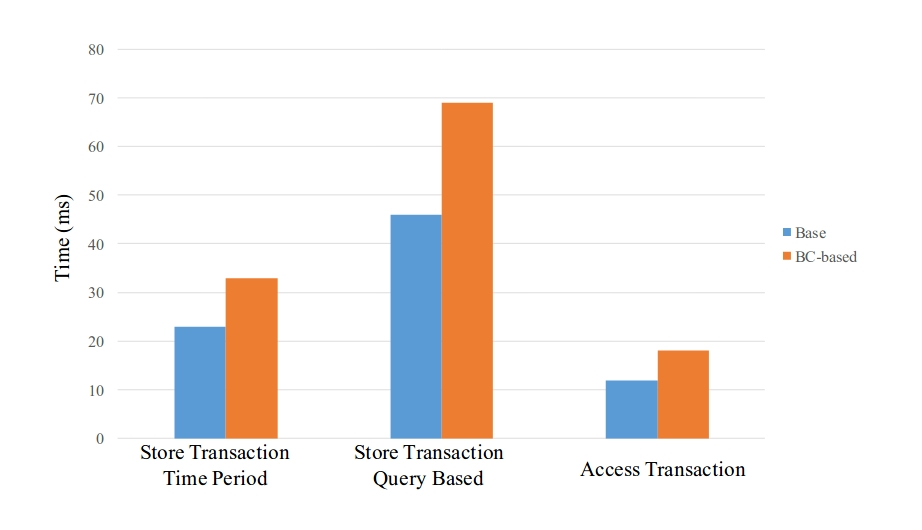
\includegraphics[width=0.8\textwidth]{pictures/results1.jpg}
        \caption{Gráfico dos dados de sobrecarga}
        \label{fig:results1}
    \end{figure}{}
    
    \item[] \textbf{Consumo de Energia}: A Figura 3 descreve os resultados de consumo de energia. Como é evidente, o projeto baseado em blockchain aumenta o consumo de energia em 0,07 (mj). A tabela na parte inferior da Figura 3 descreve o consumo de energia para as 3 tarefas centrais executadas pelo minerador: CPU, transmissão (Tx) e escuta (Lx). O consumo de energia por CPU aumentou em torno de 0,002 (mj) mp projeto devido a criptografia e hashing. A transmissão de pacotes de dados mais longos dobrou o consumo de energia de transmissão da solução utilizando em blockchain em comparação com o método que não usava. As baixas despesas gerais introduzidas pela solução que utiliza blockchain para segurança em internet das coisas superam significativamente o que não utiliza blockchain dados os significativos benefícios de segurança e privacidade oferecidos em troca de um custo não tão alto de energia.
    
    \begin{figure}[H]
        \centering
        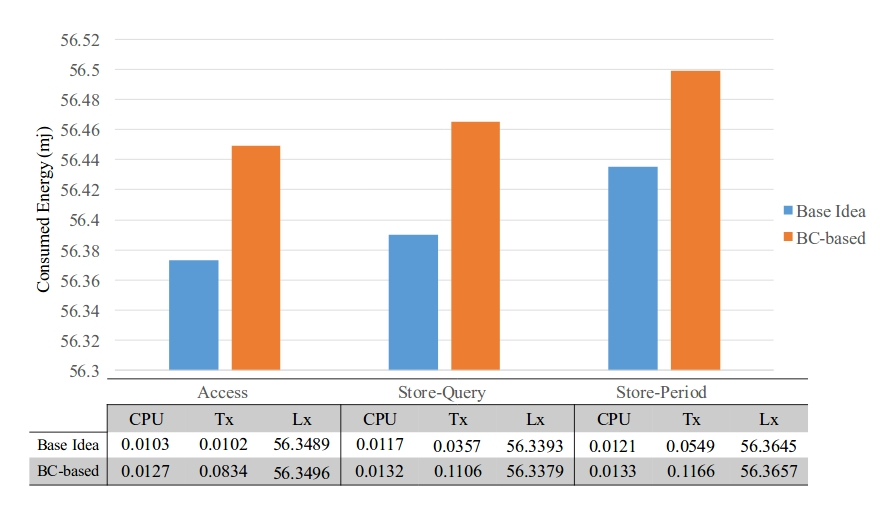
\includegraphics[width=0.8\textwidth]{pictures/results2.jpg}
        \caption{Gráfico dos dados de consumo de energia}
        \label{fig:my_label}
    \end{figure}{}
\end{itemize}{}
